\documentclass[10pt]{article}
\usepackage{acl}
\usepackage{times}
\usepackage{latexsym}
\usepackage[T1]{fontenc}
\usepackage[utf8]{inputenc}
\usepackage{microtype}
\usepackage{inconsolata}
\usepackage{enumitem}
\usepackage{url}
\usepackage{booktabs}
\usepackage{amsmath}
\usepackage{mathtools}
\usepackage{graphicx}
\usepackage{tikz}
\usetikzlibrary{arrows.meta,positioning,calc}

\setlist[itemize]{leftmargin=1.3em,itemsep=0.2em,topsep=0.2em,parsep=0em}

\title{ScholarRAG: AI-Powered Literature Assistant}

\author{
Sushil Dalavi, Parvathi Sanjana Pericherla, Eshna Gupta \\
University of Southern California \\
\texttt{\{sdalavi, pperiche, eshnagup\}@usc.edu}
}

\begin{document}
\maketitle

\begin{abstract}
Students and researchers often use AI tools to speed up literature
review, but those tools frequently produce answers that sound
convincing without making clear whether each claim is actually
supported by a paper. ScholarRAG addresses this by answering questions
over scholarly documents, attaching a citation to each generated
sentence, and estimating how reliable each cited claim appears to be.
This midterm report focuses on the NLP and LLM components of the
system: our retrieval pipeline, query disambiguation module,
citation-grounded generation protocol, and two-stage M/S/A confidence
model. At the midpoint of the semester, the core pipeline is
implemented end to end, and we have completed an initial round of
manual claim-level annotation for confidence calibration. Our current
analysis centers on preliminary logistic calibration of the M/S/A
signal blend; broader retrieval benchmarking, larger-scale answer
evaluation, ablation studies, and significance testing remain in
progress for the final paper.
\end{abstract}

\section{Introduction}

\paragraph{What we are trying to do.}
We want to build a tool that can read a set of research papers, answer
a user's question in plain language, and show exactly which paper
passage supports each part of the answer. The tool should not just
sound confident; it should make it easy for a reader to check whether
the answer is actually backed by the papers.

\paragraph{Why this matters.}
Students and researchers increasingly use AI systems to speed up
literature review, but many systems produce polished answers without
making it clear which claims are supported and which are guesses. This
is risky in academic work. If a user cannot tell where an answer came
from, they may repeat an incorrect claim in a report, design an
experiment based on a false summary of prior work, or trust a result
that was never actually stated in the cited paper.

\paragraph{Who cares and what difference it would make.}
If ScholarRAG works well, it could reduce the time needed to search
through papers while also making AI-generated summaries easier to
verify. Instead of treating an answer as a black box, users would be
able to inspect the evidence sentence by sentence and see whether the
system itself believes the cited support is strong or weak. This is
especially useful for students and early-stage researchers, who often
need help navigating unfamiliar literature but also need a clear path
to checking what is trustworthy.

This report focuses entirely on the NLP and LLM components of the
system. At the midterm stage, our main contributions are:
\begin{itemize}
    \item a retrieval pipeline for uploaded scholarly documents that
          combines dense search with lexical reranking,
    \item a query sense disambiguation module for ambiguous technical
          terms,
    \item a citation-grounded generation protocol that suppresses
          unsupported statements,
    \item a two-stage confidence model that combines retrieval signals
          with claim-level semantic match, retrieval stability, and
          agreement signals,
    \item an export-and-annotation workflow for manually labeling
          claim-evidence pairs and calibrating the confidence model.
\end{itemize}

\section{Related Work}

\paragraph{Retrieval-Augmented Generation.}
\citet{lewis2020rag} introduced RAG as a framework for grounding
generated text in retrieved documents rather than relying only on
parametric memory. Dense retrievers such as DPR
\citep{karpukhin2020dpr} improve semantic matching between queries and
documents, while token-level approaches such as ColBERT
\citep{khattab2020colbert} and later reranking work
\citep{izacard2021leveraging,gao2023rag} improve ranking quality after
initial retrieval. ScholarRAG follows this broad design, but targets
paper question answering over uploaded documents and places stronger
emphasis on evidence support and user-visible confidence.

\paragraph{Faithfulness and Attribution.}
A core weakness of RAG systems is that retrieved context does not
guarantee that the generated answer is faithful to that context.
\citet{maynez2020faithfulness} distinguish between contradictions and
unsupported additions, while \citet{min2023factscore} argue for
claim-level evaluation of long-form generation. \citet{rashkin2023attribution}
further emphasize that generated statements should be attributable to
specific evidence. ScholarRAG adopts this position directly: each
answer sentence should be traceable to a retrieved paper passage, and
unsupported claims should be suppressed rather than merely decorated
with a citation.

\paragraph{NLI and Semantic Support.}
Natural language inference has become a standard way to estimate
whether one piece of text is supported by another. In particular,
\citet{honovich2022true} show that entailment-style models are strong
proxies for factual consistency. This motivates our semantic match
signal $M$, which treats the generated claim as the hypothesis and the
cited passage as the premise:
\begin{equation}
M = P(\text{entailment} \mid \text{claim}, \text{passage})
\end{equation}
This is the most direct of our confidence signals because it asks
whether the cited passage actually supports the claim.

\paragraph{Uncertainty and Stability.}
Several works suggest that consistency under perturbation is useful as
a proxy for confidence. \citet{kuhn2023semantic} propose uncertainty
measures based on semantic perturbations, and ensemble-style
uncertainty methods such as \citet{lakshminarayanan2017simple} show
that agreement across repeated runs can reflect robustness. Our
stability signal $S$ follows this principle by asking whether the same
evidence still appears when retrieval is perturbed:
\begin{equation}
S = \frac{\# \text{ retrieval runs in which the evidence reappears}}
         {\# \text{ total retrieval runs}}
\end{equation}

\paragraph{Multi-Source Verification and Calibration.}
Multi-document verification work such as FEVER \citep{thorne2018fever},
FEVEROUS \citep{wadden2020feverous}, and HotpotQA
\citep{yang2018hotpotqa} motivates our agreement signal $A$, which
measures whether multiple independent sources support the same claim:
\begin{equation}
A = \frac{\# \text{ distinct sources supporting the claim}}
         {\# \text{ retrieved sources}}
\end{equation}
We then combine $M$, $S$, and $A$ in a logistic blend and calibrate
the weights against labeled claim-evidence pairs, following the broad
idea of model-confidence calibration \citep{guo2017calibration}.

\section{Proposed Method}

Figure~\ref{fig:pipeline} shows the current ScholarRAG pipeline.

\begin{figure}[t]
\centering
\footnotesize
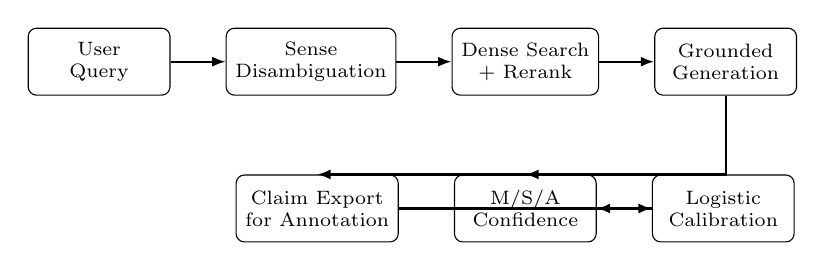
\begin{tikzpicture}[
  node distance=0.7cm and 0.7cm,
  box/.style={
    draw,
    rounded corners=3pt,
    align=center,
    minimum width=1.8cm,
    minimum height=0.85cm,
    font=\scriptsize
  },
  arr/.style={-{Latex[length=1.7mm]}, thick}
]

\node[box] (q) {User\\Query};
\node[box, right=of q] (wsd) {Sense\\Disambiguation};
\node[box, right=of wsd] (ret) {Dense Search\\+ Rerank};
\node[box, right=of ret] (gen) {Grounded\\Generation};

\node[box, below=1.0cm of ret] (conf) {M/S/A\\Confidence};
\node[box, left=of conf] (ann) {Claim Export\\for Annotation};
\node[box, right=of conf] (cal) {Logistic\\Calibration};

\draw[arr] (q) -- (wsd);
\draw[arr] (wsd) -- (ret);
\draw[arr] (ret) -- (gen);
\draw[arr] (gen.south) |- (conf.north);
\draw[arr] (gen.south) |- (ann.north);
\draw[arr] (ann) -- (cal);
\draw[arr] (cal) -- (conf);

\end{tikzpicture}
\caption{ScholarRAG NLP pipeline. A query is disambiguated, matched
against uploaded documents, answered with sentence-level citations, and
then scored by the M/S/A confidence module. Claim-evidence pairs can
also be exported for manual annotation and logistic calibration.}
\label{fig:pipeline}
\end{figure}

\subsection{Document Representation and Retrieval}

Uploaded papers are chunked into overlapping text segments and embedded
with \texttt{mxbai-embed-large} served through Ollama. We use
asymmetric query and document prefixes to reflect the fact that a user
question and a document chunk play different roles in retrieval. Each
stored embedding is tagged with its provider, model, version, and
dimension so that incompatible embeddings are not mixed at retrieval
time.

The current uploaded-document retrieval path starts with dense vector
search over the stored chunk embeddings. We then apply lexical
reranking and document-balancing heuristics so that exact technical
phrases remain important and one long document does not dominate the
candidate set in multi-document mode.

\subsection{Query Sense Disambiguation}

Before retrieval, the system applies a lightweight query sense
disambiguation module to ambiguous technical terms. Words such as
\textit{attention}, \textit{transformer}, or \textit{encoder} can mean
different things across subfields. If the system retrieves evidence for
the wrong sense, even strong generation will produce the wrong answer.
Our disambiguation step uses a curated domain lexicon and context cues
from retrieved evidence to prefer the most plausible technical sense
before final answer generation.

\subsection{Citation-Grounded Generation}

Generation is performed with GPT-4o-mini. The model receives the top
retrieved chunks and is instructed to produce an answer in which every
sentence is grounded in the provided evidence. If a statement cannot be
supported by the retrieved passages, the system is designed to omit it
rather than include it without support. In multi-document mode, the
prompt also encourages synthesis across papers while preserving
per-sentence attribution.

\subsection{Two-Stage Confidence Model}

ScholarRAG assigns a confidence estimate to cited evidence using a
two-stage design.

\paragraph{Stage 1: Retrieval-Oriented Confidence.}
The first stage uses retrieval-side signals such as similarity,
reranker strength, citation coverage, and evidence separation. These
signals provide a coarse estimate of whether the system found enough
relevant material to support a grounded answer at all.

\paragraph{Stage 2: M/S/A Evidence Confidence.}
The second stage scores each citation using three claim-level signals:
\begin{itemize}
    \item \textbf{M (Semantic Match):} how strongly the cited passage
    semantically supports the generated claim.
    \item \textbf{S (Retrieval Stability):} how consistently the same
    evidence appears under perturbed retrieval runs.
    \item \textbf{A (Agreement):} whether multiple sources or selected
    documents support the same claim.
\end{itemize}

Following our confidence-design formulation, these signals are combined
by a logistic blend:
\begin{equation}
\text{score}_2 = \sigma(b + w_1M + w_2S + w_3A)
\end{equation}

We initialize this blend with heuristic default weights
$w_1 = 0.58$, $w_2 = 0.22$, $w_3 = 0.20$, and $b = 0.0$. These values
were chosen as priors rather than learned constants: semantic match is
given the largest starting weight because it is the most direct signal
of support, while stability and agreement provide complementary but
less direct evidence. These defaults are then updated through logistic
calibration on labeled claim-evidence data.

The full system blends this M/S/A evidence score with the retrieval
confidence stage:
\begin{equation}
\text{Confidence} =
\operatorname{clamp}\bigl(
0.62\,\text{score}_1 + 0.38\,\text{score}_2
\bigr)
\end{equation}

\subsection{Annotation and Calibration Workflow}

To evaluate and calibrate the confidence model, we export system
outputs into annotation-friendly CSV files. These files contain query
text, generated answers, individual answer claims, cited evidence
spans, and the M/S/A feature values already computed by the system.
Human annotators then review each claim-evidence pair and assign a
binary label: \textit{Supported} or \textit{Unsupported}.

These annotations are converted into calibration records and passed
into a logistic regression fitting step. The learned parameters are
stored in PostgreSQL and loaded at runtime, allowing the system to use
updated calibration weights without changing the codebase.

\subsection{What Is New}

ScholarRAG differs from standard paper-question answering systems in
three ways. First, it enforces sentence-level grounding during answer
generation rather than only listing papers at the end of the answer.
Second, it produces a per-citation confidence estimate rather than a
single answer-level confidence score. Third, it learns that confidence
estimate from an interpretable three-signal decomposition --- semantic
match, retrieval stability, and agreement --- instead of relying on a
single retrieval score.

\section{Experimental Plan}
\label{sec:experiments}

\subsection{Hypotheses}

\begin{itemize}
    \item \textbf{H1:} The three M/S/A signals provide complementary
    information for determining whether a generated claim is supported
    by its cited evidence.

    \item \textbf{H2:} Logistic calibration over manually labeled
    claim-evidence pairs yields more meaningful citation confidence
    than fixed heuristic weights alone.

    \item \textbf{H3:} In the current uploaded-document setting,
    semantic match and agreement are stronger predictors of support
    than retrieval stability.
\end{itemize}

\subsection{Planned Experiments}

Our final evaluation plan has three parts.

\paragraph{Retrieval quality.}
We will run user-style queries over an uploaded paper corpus and
measure whether the system retrieves the correct supporting documents
and chunks.

\paragraph{Answer faithfulness.}
We will evaluate whether generated claims are actually supported by the
cited passages through structured annotation and expanded judge-based
review.

\paragraph{Confidence calibration.}
We will export claim-evidence pairs, collect support labels, fit
logistic regression over the M/S/A features, and analyze whether the
learned weights align with our intuitions about evidence quality.

\subsection{Evaluation Plan}

For the final paper, retrieval quality will be evaluated with ranking
metrics such as Recall@K, MRR, and nDCG. Faithfulness will be
evaluated through claim-level support judgments and citation coverage.
Confidence calibration will be evaluated on held-out labeled data using
calibration-oriented metrics such as Brier score and related
correlation analyses.

In this midterm report, however, we do not present finalized retrieval
or faithfulness metrics because those broader experiments are still in
progress. Instead, we focus on the part of the workflow that is
already complete end to end: claim-level annotation and preliminary
M/S/A calibration.

\section{Preliminary Results}

At the midpoint of the project, the full retrieval-to-generation
pipeline is operational for the NLP/LLM components, and the M/S/A
confidence workflow is implemented end to end. We have completed an
initial round of manual claim-level annotation and used those labels to
fit a preliminary logistic calibration model over the three M/S/A
signals.

\subsection{Calibration Dataset Snapshot}

Our current labeled set contains 634 claim-evidence pairs annotated as
either \textit{Supported} or \textit{Unsupported}. Table~\ref{tab:head}
shows the first five rows of the current claim-annotation dataset in a
compact form.

\begin{table*}[t]
\centering
\small
\begin{tabular}{lllllll}
\toprule
Query ID & Claim ID & Claim excerpt & $M$ & $S$ & $A$ & Label \\
\midrule
q1 & q1\_c1 & I only found the requested topic mentioned in profile/course context. & 0.0968 & 0.25 & 0.00 & unsupported \\
q1 & q1\_c2 & I do not have enough reliable evidence here to give a broad definition. & 0.0914 & 0.45 & 0.00 & unsupported \\
q3 & q3\_c1 & I only found the requested topic mentioned in context rather than as support. & 0.1000 & 0.55 & 0.00 & unsupported \\
q3 & q3\_c2 & I do not have enough reliable evidence here to give a broad definition. & 0.0914 & 0.35 & 0.00 & unsupported \\
q9 & q9\_c1 & The answer incorrectly reframed the RAG paper as a misbehavior-reduction system. & 0.1600 & 0.55 & 0.00 & unsupported \\
\bottomrule
\end{tabular}
\caption{Head(5) of the current claim-annotation dataset, shown in a
compact form for readability. The first five rows happen to be
unsupported examples, which reflects early failure cases in the current
annotation file.}
\label{tab:head}
\end{table*}

\subsection{Preliminary M/S/A Calibration}

Using these labels, we fit logistic regression over semantic match
($M$), retrieval stability ($S$), and agreement ($A$). The resulting
preliminary weights are shown in Table~\ref{tab:weights}.

\begin{table}[t]
\centering
\small
\begin{tabular}{lc}
\toprule
Parameter & Value \\
\midrule
$w_1$ (semantic match) & 3.55 \\
$w_2$ (retrieval stability) & 0.18 \\
$w_3$ (agreement) & 4.93 \\
$b$ (bias) & -2.76 \\
\bottomrule
\end{tabular}
\caption{Preliminary logistic calibration weights learned from the
current labeled claim-evidence set.}
\label{tab:weights}
\end{table}

This yields the following preliminary calibrated M/S/A blend:
\begin{equation}
\widehat{\text{score}}_2 =
\sigma(-2.76 + 3.55M + 0.18S + 4.93A)
\end{equation}

The learned weights suggest that, on the current annotation set,
semantic match and agreement are the strongest signals, while retrieval
stability adds less additional separation. Unsupported claims tend to
have very weak semantic support from the cited passage, while supported
claims usually combine strong entailment with strong agreement from the
selected evidence.

To better understand this pattern, Table~\ref{tab:msa-by-label}
compares mean M/S/A values across the two label groups.

\begin{table}[t]
\centering
\small
\begin{tabular}{lcccc}
\toprule
Label & Count & $M$ & $S$ & $A$ \\
\midrule
Supported & 570 & 0.80 & 0.84 & 1.00 \\
Unsupported & 64 & 0.07 & 0.52 & 0.00 \\
\bottomrule
\end{tabular}
\caption{Mean M/S/A values for the current manually labeled
claim-evidence pairs.}
\label{tab:msa-by-label}
\end{table}

The strongest separation is in $A$: on the current set, supported
claims almost always receive high agreement, while unsupported claims
receive none. This makes agreement especially powerful in the present
data. At the same time, this is also a warning that the current
weights should be treated as preliminary rather than final. The
annotation set is still relatively narrow and includes many
single-document questions, so the learned values are likely to reflect
the current dataset structure as much as general evidence quality.

\subsection{Interpretation of the Preliminary Weights}

The current fit supports two early conclusions. First, the M/S/A
decomposition is meaningful: the three signals do not behave randomly,
and supported versus unsupported claims occupy clearly different
regions of feature space. Second, semantic match and agreement appear
to carry most of the predictive burden in the current data, which is
exactly the kind of interpretable behavior we wanted from the model.

However, the present results are not yet a final calibration study.
They were fit on the current labeled dataset itself rather than on a
held-out evaluation split, and the current claim set is not yet broad
enough to ensure that the learned weights are stable across task types.
For that reason, we treat these numbers as an initial empirical
calibration of the model design rather than definitive task-wide
weights.

\subsection{Current Status of Broader Evaluation}

The broader evaluation pipeline is partially implemented but not yet
ready to report final quantitative results. In particular, larger-scale
retrieval benchmarking, broader faithfulness measurement, ablation
studies, and significance testing remain future work. Our strongest
midterm result is therefore not a final benchmark score, but the fact
that the confidence-calibration workflow is now operational and already
produces interpretable learned weights from human labels.

\section{Milestone Progress}

\subsection{Original Milestones}

Our project proposal set two main midterm milestones:
\begin{itemize}
    \item \textbf{Milestone 1:} Build a working end-to-end system with
    retrieval, citation-grounded generation, and inline citations.
    \item \textbf{Milestone 2:} Design and integrate a confidence
    scoring module together with a realistic plan for quantitative
    evaluation.
\end{itemize}

\subsection{Progress Against Milestones}

We are substantially on track for both milestones. For Milestone 1, the
retrieval pipeline, query disambiguation module, citation-grounded
generation, and multi-document answer flow are implemented and
functional. The system can ingest papers, search across them, generate
answers with sentence-level citations, and export claim-evidence pairs
for inspection.

For Milestone 2, the two-stage M/S/A confidence model is fully
integrated. More importantly, the surrounding evaluation workflow is
now in place: we can export annotation files, collect support labels,
fit logistic regression over M/S/A features, store learned weights, and
reuse those weights during later inference.

The remaining work is mostly evaluative rather than infrastructural.
We still need broader held-out experiments, larger-scale annotations,
ablation studies, and statistical testing, but the core mechanism we
set out to build is already operational.

\subsection{Updated Milestones for the Remainder of the Semester}

\begin{itemize}
    \item \textbf{Week 10:} Expand the open-corpus query set and add
    more diverse multi-document prompts and harder support cases.

    \item \textbf{Week 11:} Continue manual labeling of claim-evidence
    pairs and strengthen the answer-review workflow for faithfulness
    evaluation.

    \item \textbf{Week 12:} Refit logistic regression over the expanded
    M/S/A annotation set and run ablations to test the contribution of
    each feature.

    \item \textbf{Week 13:} Add held-out evaluation, significance
    testing, and error analysis for unsupported and borderline cases.

    \item \textbf{Week 14:} Finalize the report, polish the system
    demonstration, and present end-to-end results.
\end{itemize}

\section{Conclusion}

ScholarRAG is motivated by a simple goal: AI answers about research
papers should be easy to verify, not merely easy to read. Our system
tries to do this by retrieving evidence from uploaded papers,
generating cited answers, and attaching an interpretable confidence
estimate to each cited claim.

At the midpoint of the semester, the most concrete progress is that the
M/S/A calibration workflow is now complete end to end. We can export
claim-evidence pairs, label them manually, fit logistic weights over
semantic match, retrieval stability, and agreement, and feed those
weights back into the running system. Preliminary fitted weights
suggest that semantic match and agreement are especially important on
the current dataset, while retrieval stability provides a weaker but
still useful secondary signal.

The remaining work is to broaden and validate these findings. We still
need held-out calibration evaluation, broader retrieval and
faithfulness experiments, and more detailed ablation studies. If
successful, ScholarRAG will provide a practical research assistant in
which every answer is not only cited, but also accompanied by a
transparent estimate of how strongly the available evidence supports
it.

\bibliography{custom}
\bibliographystyle{acl_natbib}

\end{document}
